%!TEX root = ../book.tex
\section{Coordinate Systems and Frames of Reference}\label{sec:coordsystems}

\screencast{http://youtu.be/klBJi-MEeNQ}{coordinatesystem}

Every robot assumes a \textsl{pose}\index{Pose} in the real world that can be described by its position ($x$, $y$ and $z$) and orientation (pitch, yaw and roll) along the three major axes of a Cartesian Coordinate system (see also \cref{sec:dof}).
Such a coordinate system is shown in \cref{fig:coordinatesystem}. Note that the directions and orientations of the coordinate axes are arbitrary. This book uses the ``right hand rule'', which is illustrated in \cref{fig:coordinatesystem} to determine axes labels and directions throughout.
Pitch, yaw, and roll, are also known as bank, attitude, and heading in other communities\index{Pitch}\index{Yaw}\index{Roll}\index{Bank}\index{Attitude}\index{Heading}. This makes sense, considering the colloquial use of the word ``heading'', which corresponds to a rotation around the $z-$axis of a vehicle driving on the $x-y-$plane.

\begin{figure}
    \centering
    % 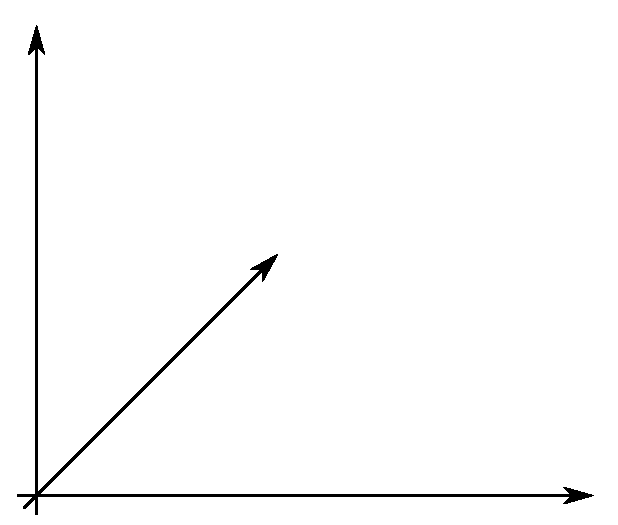
\includegraphics[width=0.8\textwidth]{figs/coordinatesystem}
    \def\svgwidth{0.8\textwidth}
    \import{./figs/kinematics/}{coordinatesystem.pdf_tex}
    \caption{A coordinate system indicating the direction of the coordinate axes and rotation around them. These directions have been derived using the right-hand rules.}
    \label{fig:coordinatesystem}
\end{figure}

Defining all three position axes and orientations might be cumbersome. What level of detail we care about, where the origin of this coordinate system is, and even what kind of coordinate system we choose, depends on the specific application.
For example, a simple mobile robot would typically require a representation with respect to a room, a building, or the earth's coordinate system (given by the longitude and latitude of each point on earth), whereas a static manipulator usually has the origin of its coordinate system at its base.
More complicated systems, such as mobile manipulators or multi-legged robots, make life much easier by defining multiple coordinate systems, e.g.\ one for each leg and one that describes the position of the robot in the world frame. These local coordinate systems are known as \emph{Frames of Reference}\index{Frame of Reference}.
An example of two nested coordinate systems is shown in \cref{fig:nestedcoords}. In this example, a robot located at the origin of $x',y'$ and $z'$ might plan its motions in its own reference frame, which can then be expressed in the coordinate system $x$, $y$ and $z$ by performing a translation and a rotation---as we will later see.

Depending on its degrees of freedom in Cartesian space---that is, the number of independent translations and rotations a robot can achieve in such a space---it is also customary to ignore components of position and orientation that remain constant.
For example, a simple floor-cleaning robot's pose might be completely defined by its $x$ and $y$ coordinates in a room as well as its orientation, i.e.\ its rotation around the $z$-axis. In this case, $z$ position and rotation around $x$ and $y$ axes would be ignored.

\begin{figure}
    \centering
    %
\includegraphics[width=\textwidth]{figs/frameofreference.png}
    \def\svgwidth{\textwidth}
    \import{./figs/kinematics/}{nestedcoords.pdf_tex}
    \caption{Two nested coordinate systems (also referred to as frames of reference).}
    \label{fig:nestedcoords}
\end{figure}

\subsection{Matrix notation}
Given some kind of fixed coordinate system, we can describe the \emph{position} of a robot's end-effector by a $3\times1$ position vector.
As there can be many coordinate systems defined on a robot and the environment, we identify the coordinate system a point relates to by a preceeding super-script, e.g., $ ^AP$ to indicate that point $P$ is in coordinate system $\{A\}$.
Each point consists of three elements $ ^AP=[p_x, p_y, p_z]^T$.

More formally, $^AP$ is a linear combination of the three basis vectors that span $A$:
\begin{equation}
^AP=p_x\left[\begin{array}{c}1\\0\\0\end{array}\right]+p_y\left[\begin{array}{c}0\\1\\0\end{array}\right]+p_z\left[\begin{array}{c}0\\0\\1\end{array}\right]\label{eq:basis}
\end{equation}

\screencast{http://youtu.be/QdHO_9M8-UI}{frameofreference}

As we know, not only the position of the robot is important, but also its orientation.
In order to describe the orientation of a point, we will attach a coordinate system to it. Let $ \hat{X}_B, \hat{Y}_B$ and $ \hat{Z}_B$ be unit vectors that correspond to the principal axes of a coordinate system $\{B\}$.
When expressed in coordinate system $\{A\}$, they are denoted $^A\hat{X}_B, ^A\hat{Y}_B$ and $ ^A\hat{Z}_B$.
In order to express a vector that is given in one coordinate system in another, we need to \textsl{project} each of its components to the unit vectors that span the target coordinate system. For example, if we consider only the axis $^A\hat{X}_B$, we have that:

\begin{equation}\label{eq:projection}
^A\hat{X}_B=(\hat{X}_B\cdot\hat{X}_A, \hat{X}_B\cdot\hat{Y}_A,\hat{X}_B\cdot\hat{Z}_A)^T
\end{equation}

consists of the projections of $\hat{X}_B$ onto $\hat{X}_A$, $\hat{Y}_A$ and $\hat{Z}_A$. Here, `$\cdot$' denotes the scalar product (also known as dot or inner product, see \cref{app:linalg:dotproduct}).
Note that all vectors in (\ref{eq:projection}) are unit vectors, i.e.\ their length is one.
By following the definition of the scalar product, we have that $A\cdot B=\|A\|\|B\|\cos \alpha=\cos \alpha$, indeed reduces the projection of $\hat{X}_B$ onto the unit vectors of $\{A\}$. This projection is illustrated in \cref{fig:projection}.

\begin{figure}
    \centering
    % 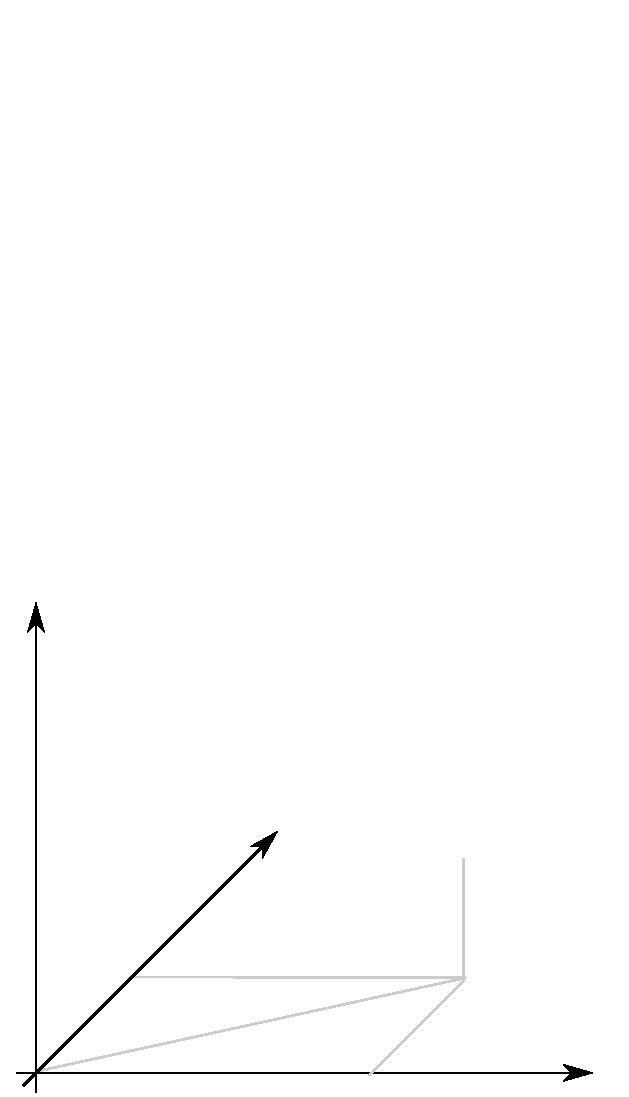
\includegraphics[width=0.8\textwidth]{figs/projection.png}
    \def\svgwidth{0.8\textwidth}
    \import{./figs/kinematics/}{projection.pdf_tex}
    \caption{Top: A coordinate system $\{B\}$ with position given by $^AP$ and orientation given by $\hat{X}_B$, $\hat{Y}_B$, and $\hat{Z}_B$. Bottom:
    The projection of the unit vector $\hat{X}_B$ onto the unit vectors that span coordinate system $\{A\}$ after moving $\{B\}$ into the origin of $\{A\}$. As all vectors are unit vectors, $A\cdot B=\|A\|\|B\|\cos \alpha=\cos \alpha$. }
    \label{fig:projection}
\end{figure}

We can now apply the same procedure to all three vectors that span coordinate system $\{B\}$ and stack these three vectors together into a $3\times3$ matrix to obtain the rotation matrix
%
\begin{equation}
^A_BR=[^A\hat{X}_B \quad ^A\hat{Y}_B \quad ^A\hat{Z}_B]   ,
\end{equation}
%
which describes $\{B\}$ relative to $\{A\}$.
It is important to note that all columns in $ ^A_BR$ are unit vectors, so that the rotation matrix is orthonormal.
This is important as it allows us to easily obtain the inverse of $ ^A_BR$ as $ ^A_BR^T$ or
$ ^B_AR=^A_BR^T$.

The reason for which the unit vectors of a coordinate system $\{B\}$ expressed in coordinate system $\{A\}$ actually make up a rotation matrix can be easily seen when re-arranging Equation~\ref{eq:basis} in matrix form:
\begin{equation}
^AP=\left[ \arraycolsep=2pt%\def\arraystretch{2.2}
\begin{array}{ccc}1 & 0 & 0\\0 & 1 & 0\\0 & 0 & 1\end{array}\right]\left[\begin{array}{c}p_x\\p_y\\p_z\end{array}
\right],
\end{equation}
where the rotation matrix is nothing but the identity as both points already are in the same coordinate system. In this case, an identity matrix would signify a lack of rotation around all axes.

We have now established how to express the orientation of a coordinate system using a rotation matrix. Usually, coordinate systems don't lie on top of each other, but are also displaced from each other.
Together, position and orientation are known as a \emph{frame},\index{Frame} which is a set of four vectors, one for the position and three for the orientation, and we can write
%
\begin{equation}
\{B\}=\{^A_BR, ^AP\}
\end{equation}
%
to describe the coordinate frame $\{B\}$ with respect to $\{A\}$ using a vector $^AP$ and a rotation matrix $^A_BR$. Robots usually have many such frames defined along their bodies.

\subsection{Mapping from one frame to another}

\screencast{http://youtu.be/NsiJNvsuO3s}{rotationmatrix}

Having introduced the concept of frames, we need the ability to map coordinates in one frame to coordinates in another frame. For example, let's consider frame $\{B\}$ having the same orientation as frame $\{A\}$ and sitting at location $^AP$ in space. As the orientation of both frames is the same, we can express a point $ ^BQ$ in frame $\{A\}$ as:
%
\begin{equation}
^AQ=^BQ+^AP
\end{equation}
%
In reality, adding two vectors that are in different reference frames, i.e., $ ^BQ+^AP$, is only possible if both of them have the same orientation. We can, however, convert from one reference frame to the other using the rotation matrix:

\begin{equation}
^AP=^A_BR^BP
\end{equation}
%
and therefore solve the mapping problem regardless of the orientation of $\{A\}$ to $\{B\}$:
\begin{equation}
^AQ=^A_BR^BQ+^AP
\end{equation}
Using this notation, we can see that leading subscripts cancel the leading superscripts of the following vector/rotation matrix.
Even though we have now a solution to transform a point from one frame of reference to another by combining a rotation and a translation, it would be more appealing to write it in a more compact form, i.e.:
\begin{equation}
^AQ=^A_BT^BQ
\end{equation}
In order to do this, we need to introduce a $4\times1$ position vector such that
\begin{equation}
\left[\begin{array}{c}^AQ\\1\end{array}\right]=\left[\arraycolsep=2pt\begin{array}{ccc|c} & ^A_BR & & ^AP \\\hline 0 & 0 & 0 & 1\end{array}\right]\left[\begin{array}{c}^BQ\\1\end{array}\right]
\end{equation}
and $^A_BT$ is a $4\times4$ matrix.  Note that the added `$1$'s and $ [0\ 0\ 0\ 1]$ do not affect the other entries in the matrix during matrix multiplication. A $4\times4$ matrix of this form is called a \emph{homogeneous transform}.\index{Homogeneous Transform}

The inverse of an homogeneous transform can be constructed by inverting rotation and translation part independently, leading to
\begin{equation}
\left[\arraycolsep=2pt\begin{array}{ccc|c} & ^A_BR & & ^AP \\\hline 0 & 0 & 0 & 1\end{array}\right]^{-1}=
\left[\arraycolsep=2pt\begin{array}{ccc|c} & ^A_BR^T & & -^A_B{R^T}{^AP} \\\hline 0 & 0 & 0 & 1\end{array}\right]
\end{equation}

We have now established a convenient notation to convert points from one coordinate system to another. There are many possible ways this can be done, in particular how rotation can be represented (see below), but all can be converted from one into the other.

\subsection{Concatenation of Transformations}\label{sec:kinematics:coordsystems:concatenation}

Transformations can be combined: consider for example an arm with two links, reference frame $\{A\}$ at the base, $ \{B\} $ at its first joint, and $\{C\}$ at its end-effector. Given the transforms $ ^B_CT$ and $ ^A_BT$, we can write
\begin{equation}
^AP=^A_BT^B_CT^CP=^A_CT^CP
\end{equation}
to convert a point in the reference frame of the end-effector to that of its base. As this works for rotation and translation operators independently, we can construct $ ^A_CT$ as
\begin{equation}
^A_CT=\left[\arraycolsep=2pt\begin{array}{ccc|c} & ^A_BR^B_CR & & ^A_BR^BP_C +^AP_B \\\hline 0 & 0 & 0 & 1\end{array}\right]
\end{equation}
%
where $ ^AP_B$ and $ ^BP_C$ are the translations from $\{A\}$ to $\{B\}$ and from $ \{B\}$ to $\{C\}$, respectively.

\subsection{Other representations for orientation}

So far, we have represented orientation by a $3\times3$ matrix whose column vectors are orthogononal unit vectors describing the orientation of a coordinate system. Orientation is therefore represented with nine different values. We chose this representation mainly because it is the most intuitive to explain and is derived from simple geometry.

In fact, three values are sufficient to describe orientation.
This becomes clear when considering that orthogonality (dot product of all columns is zero) and vector length (each vector must have length $1$) impose six constraints on the nine values in the rotation matrix.
Indeed, an orientation can be represented as a rotation by certain angles around the $x-$, the $y-$, and the $z$-axis of the reference coordinate system. This is known as the X-Y-Z fixed-angle notation.\index{Fixed angle notation} Mathematically, this can be represented by a rotation matrix of the form:
\begin{equation}
^A_BR_{XYZ}(\gamma,\beta,\alpha)=\begin{bsmallmatrix}cos\alpha & -sin\alpha & 0\\sin\alpha & \cos\alpha & 0\\0 & 0 & 1\end{bsmallmatrix}\begin{bsmallmatrix}cos\beta& 0 & sin\beta\\0 & 1 & 0\\-sin\beta & 0 & cos\beta\end{bsmallmatrix}\begin{bsmallmatrix}1 & 0 & 0 \\ 0 & cos\gamma & -sin\gamma\\0 & sin\gamma & cos\gamma\end{bsmallmatrix}
\end{equation}

While the $X-Y-Z$ fixed angles approach expresses a coordinate frame using rotations with respect to the original coordinate frame (say, $\{A\}$), another possible description is to start with a coordinate frame $\{B\}$ that is coincident with frame $\{A\}$, then rotate around the Z-axis with angle $ \alpha$, then the Y-axis with angle $ \beta$ and finally around the X-axis with angle $ \gamma$. This representation is called Z-Y-X Euler angles.\index{Euler angles}
As the coordinate axis do not necessarily need to be different, there are twelve possible valid combinations of sub-sequent rotations: XYX, XZX, YXY, YZY, ZXZ, ZYZ, XYZ, XZY, YZX, YXZ, ZXY and ZYX.
The reason for which there are only twelve is that sub-sequent rotations around the same axis are not valid. Such rotations would not add any information, but are equivalent to a rotation by the sum of both angles.

It is important to know about the subtle differences between the available transformations as there is neither ``right'' nor ``wrong'' convention, however different manufacturers and fields use different ones.
There is only one caveat: each of the rotation matrices can look like subsequent rotations around the same axis for certain values of angles. For example, this happens for the XYZ rotation matrix if the angle of rotation around the Y-axis is $90^\circ$. These cases are known as a \emph{singularities} of the specific notation.\index{Singularity}

Among the many conventions, the preferred representation for computational and stability reasons are \emph{quaternions}\index{Quaternion}.
A quaternion is a 4-tuple that extends the complex numbers with very general applications in mathematics and representing orientation and rotation in particular. The basic idea is that each rotation can be represented as a rotation around a single axis (a vector in space) by a specific angle. Given such an axis $ \hat{K}=[k_x k_y k_z]^T$ and an angle $ \theta$, one can calculate the so-called Euler parameters\index{Euler parameters} or unit quaternion\index{unit quaternion}:

\begin{eqnarray}
\epsilon_1=k_x sin \frac{\theta}{2}\\
\epsilon_2=k_y sin \frac{\theta}{2}\\
\epsilon_3=k_z sin \frac{\theta}{2}\\
\epsilon_4=cos\frac{\theta}{2}
\end{eqnarray}

These four quantities are constrained by the relationship
\begin{equation}
\epsilon_1^2+\epsilon_2^2+\epsilon_3^2+\epsilon_4^2=1,
\end{equation}
which might be visualized by a point on a unit hyper-sphere. %Transformations are represented by \emph{dual quaternions}\index{Dual quaternion}, one for the translation and one for the rotation. Dual quaternions can again easily be converted into homogenous transformation matrices.
Analogous to rotation matrices, two quaternions $\epsilon$ and $\epsilon'$ can be multiplied using the following equation
\begin{equation}
\left[
\begin{array}{cccc}
\epsilon_4 & \epsilon_1 & \epsilon_2 & \epsilon_3\\
-\epsilon_1 & \epsilon_4 & -\epsilon_3 & \epsilon_2\\
-\epsilon_2 & \epsilon_3 & \epsilon_4 & -\epsilon_1\\
-\epsilon_3 & -\epsilon_2 & \epsilon_1 & \epsilon_4
\end{array}
\right]
\left[\begin{array}{c}\epsilon_4'\\\epsilon_1'\\\epsilon_2'\\\epsilon_3'\end{array}\right]
\end{equation}

Unlike multiplying two rotation matrices, which requires 27 multiplications and 18 additions, multiplying two quaternions only requires 16 multiplications and 12 additions, making the operation computationally more efficient.
Importantly, this representation does not suffer from singularities for specific joint angles, making the approach computationally more robust. This is particularly relevant for robotics, as mathematical singularities have pretty significant real-world impact on physical robots (see e.g. \cref{sec:invjac}).

Why any rotation can be expressed by a single vector can be seen when considering the properties of orthonomal rotation matrices. They have three eigenvalues $\lambda=1$ and a complex pair $\lambda_{1,2}=\cos \theta \pm i \sin \theta$.
Eigenvalues and eigenvectors are defined as $Rv=\lambda v$. For the case of $\lambda=1$, the corresponding Eigenvector $v$ is unchanged by rotation. This is only possible if $v$ is the actual axis of rotation.
The angle of rotation is now given by $\theta$, which can be inferred from the complex pair.
